\section{РАЗРАБОТКА ПРОГРАММНОГО ПРОДУКТА}

\subsection{Высокоуровневая архитектура}

Подводка к архитектуре.
На рисунке ~\ref{neuro_model} представлена общая арихетктура продукта.

\begin{figure}
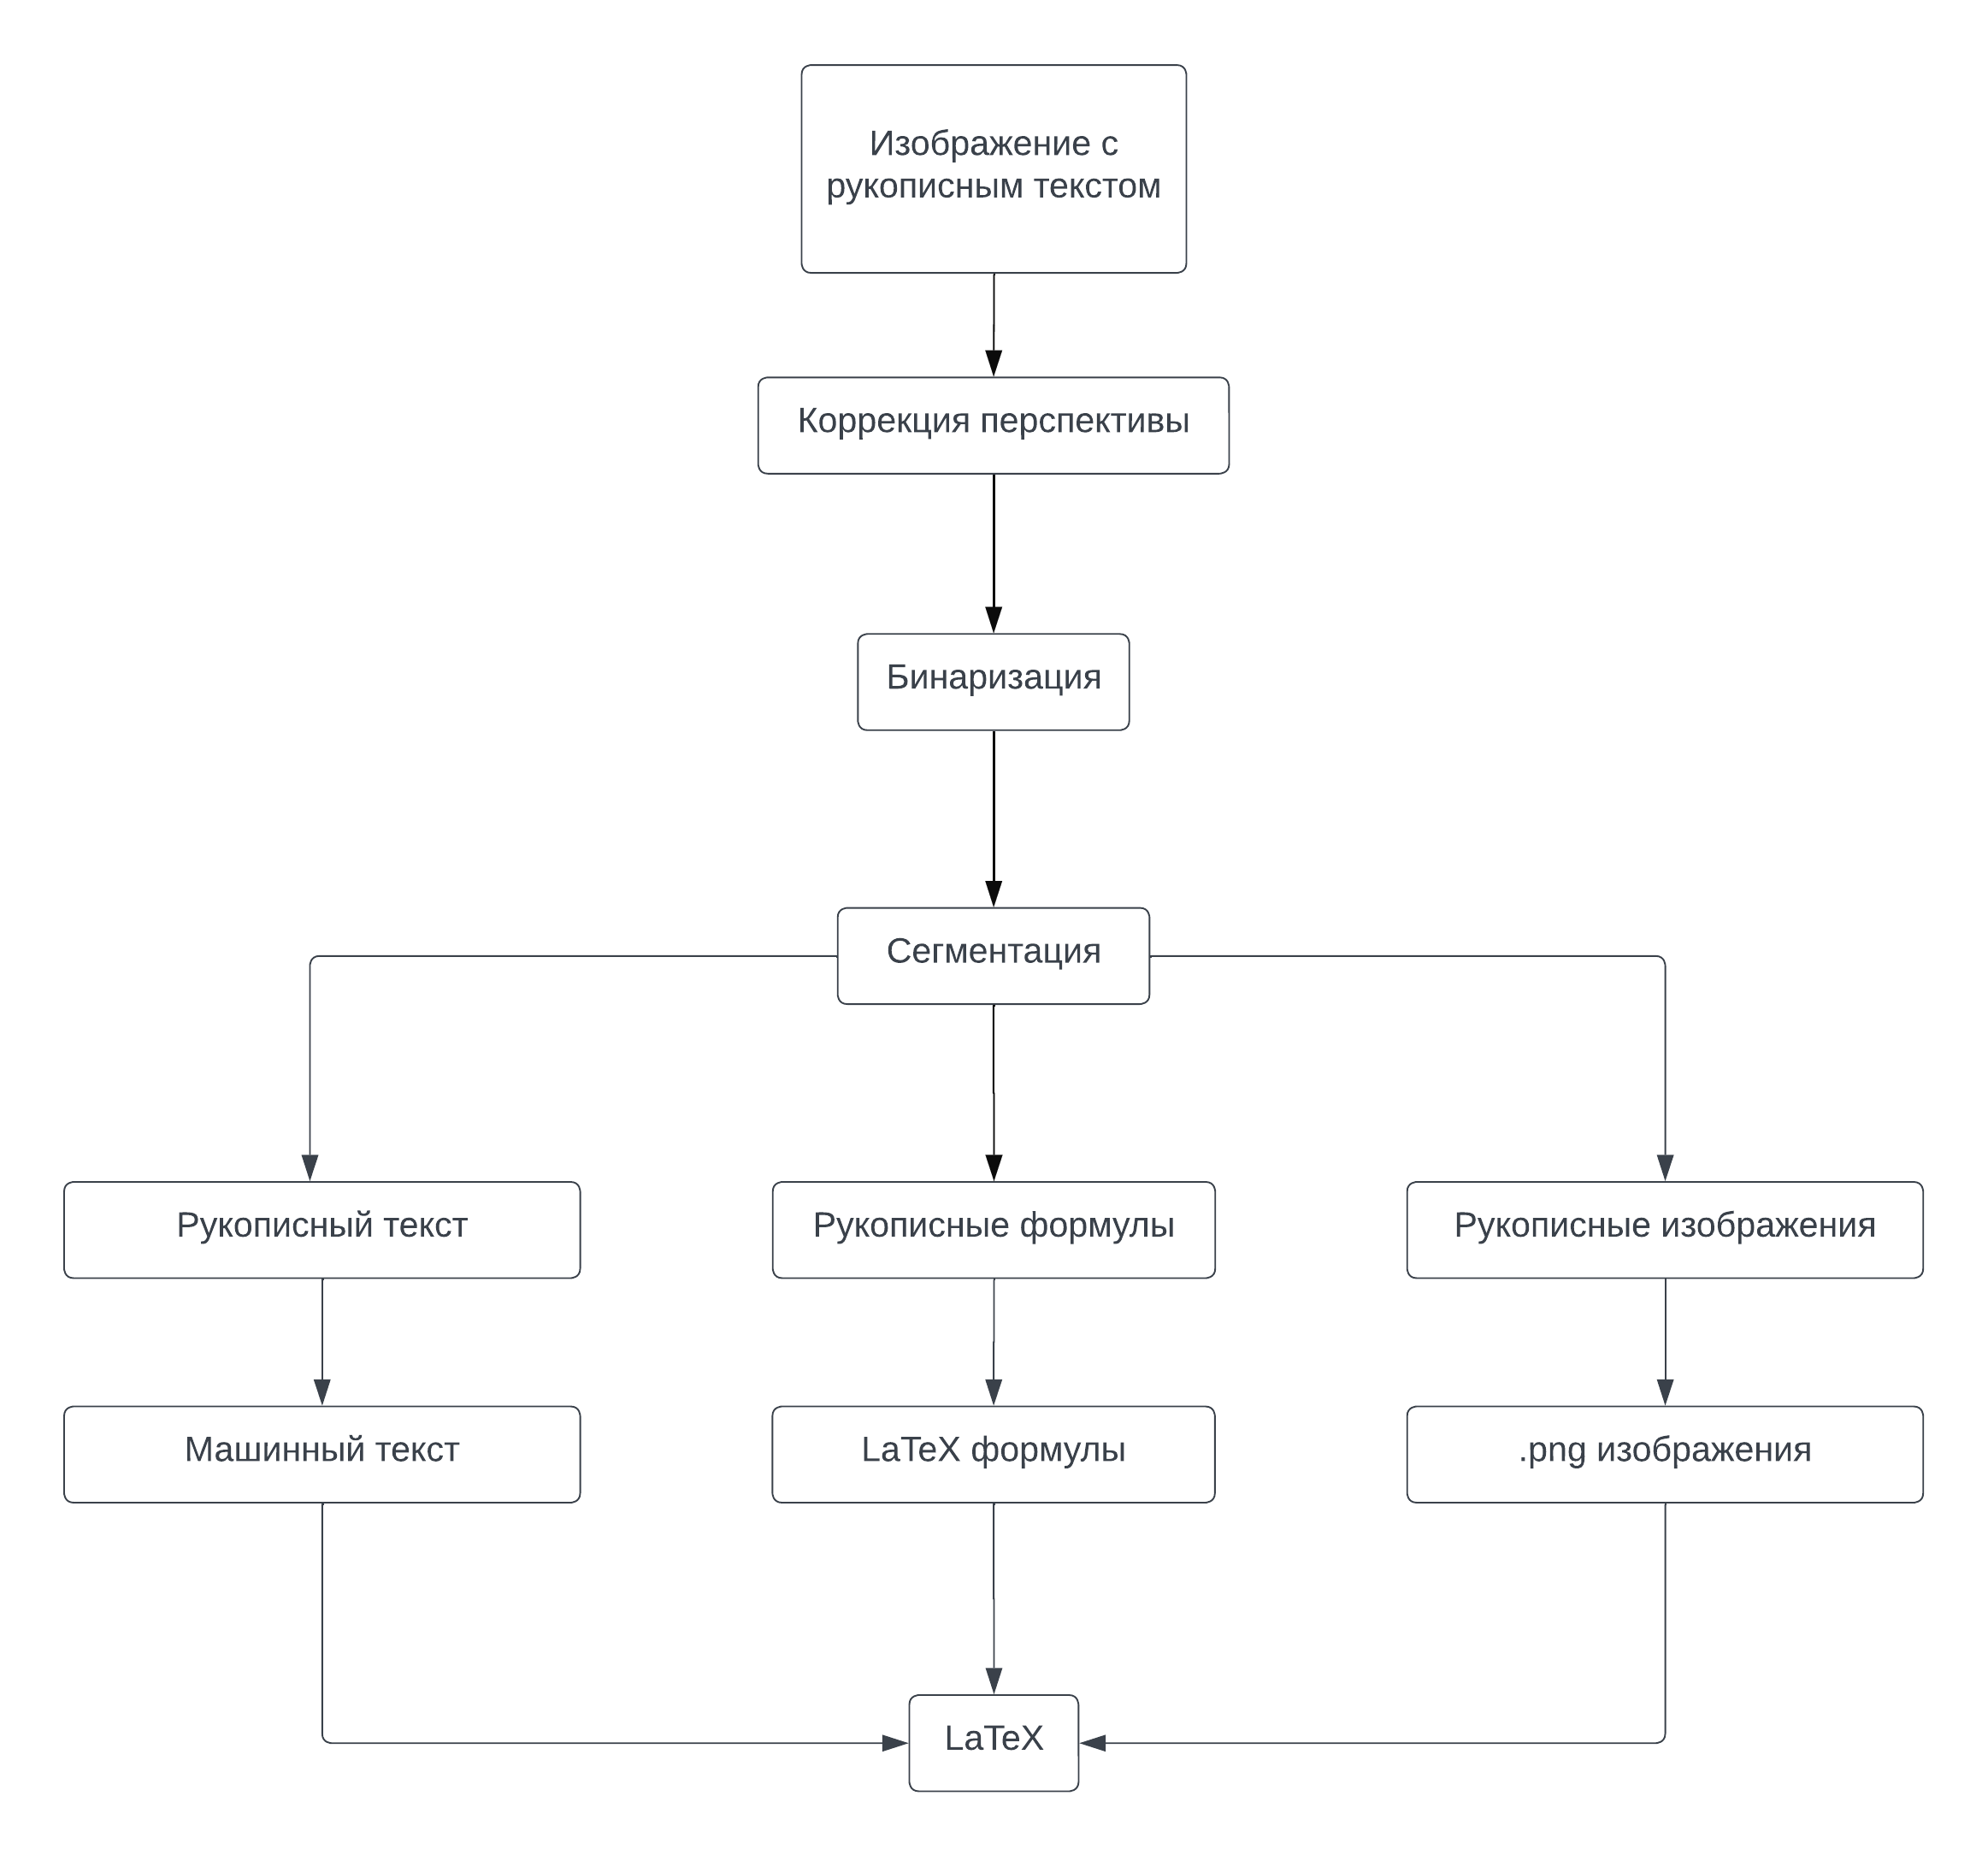
\includegraphics[scale=0.75]{img/Blank_diagram.png}
\caption{Общая архитектура модели}
\label{neuro_model}
\end{figure}

\subsection{Коррекция перспективы}

Коррекция перспективы необходима для устранения шума на изображении и получения лучшего результата. Она состоит из нескольких этапов, представленных на рисунке ~\ref{perspective_correction_algo}. 
Также на рисунке представлены результаты, получаемые на каждом из этапов обработки.

\begin{figure}
    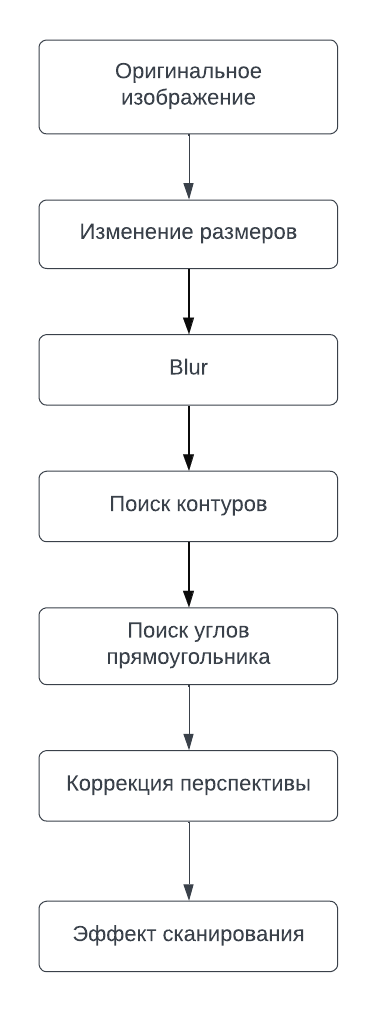
\includegraphics[scale=0.75]{img/perspective_correction}
    \caption{Этапы коррекции перспективы изображения}
    \label{perspective_correction_algo}
\end{figure}

На начальном этапе мы имеем изображение, показанное на рисунке ~\ref{input}

\begin{figure}
    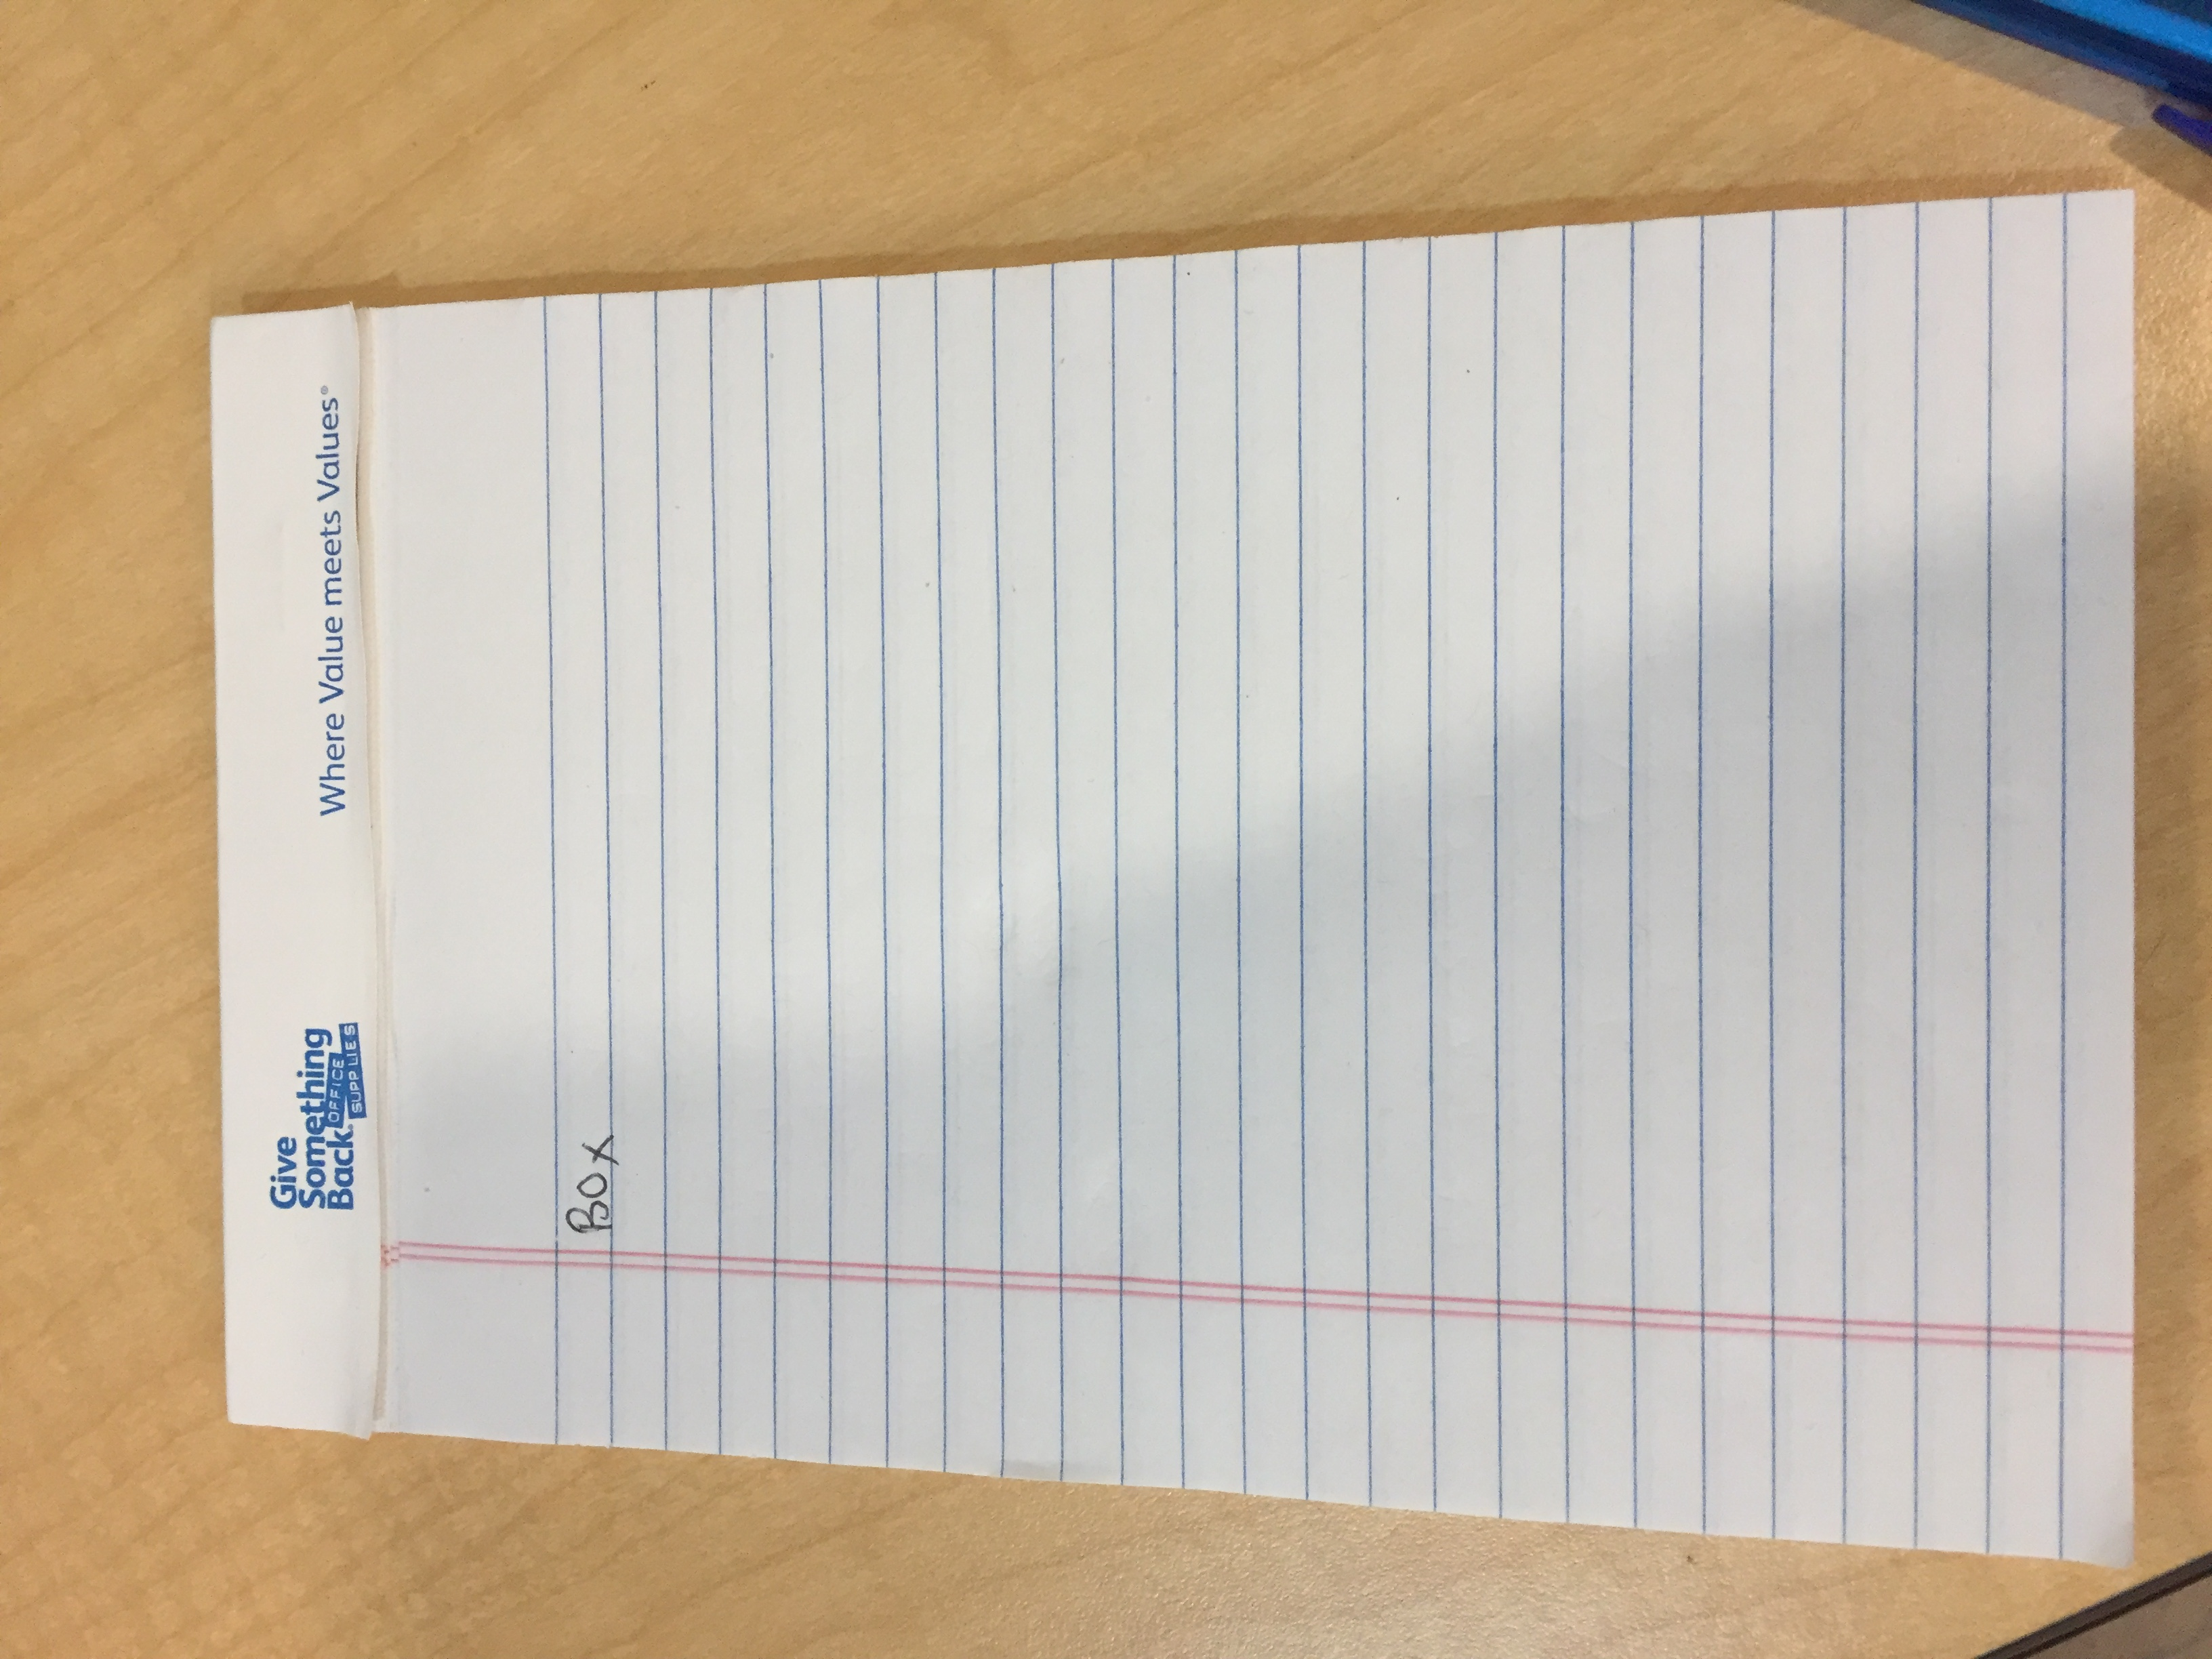
\includegraphics[scale=0.15]{img/perspective/input}
    \caption{Начальное изображение}
    \label{input}
\end{figure}

Для начала необходимо удалить текст с изображения. Для этого преобразуем изображение в серый цвет и применим к нему размытие Гаусса \cite{gauss_blur}. На выходе данного этапа имеем изображение, представленное на рисунке ~\ref{gauss_blur}

\begin{figure}
    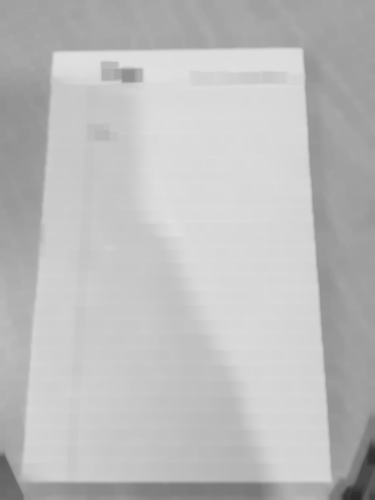
\includegraphics[scale=0.5]{img/perspective/blured.png}
    \caption{Изображение после размытия Гаусса}
    \label{gauss_blur}
\end{figure}

Для поиска контуров необходимо выделить ребра. Для этого используется алгоритм Канни \cite{canny}. На выходе имеем изображение, представленное на рисунке ~\ref{canny}
\begin{figure}
    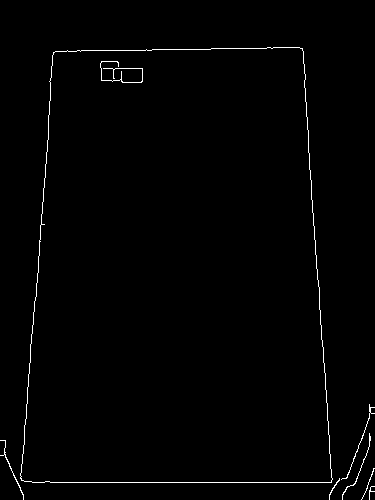
\includegraphics[scale=0.5]{img/perspective/canny}
    \caption{Ребра, найденные на изображении}
    \label{canny}
\end{figure}

После нахождения ребер поиск контуров осуществляется двумя способами:
\begin{enumerate}
    \item С помощью алгоритма $Line Segment Detector$ \cite{lsd}
    \item С помощью встроенного в $openCV$ алгоритма поиска контуров \cite{opencv_contours}
\end{enumerate}

Опишем подробнее поиск контуров на основе найденных линий: после прохода алгоритма имеем изображение, представленное на рисунке ~\ref{lsd_img}
\begin{figure}
    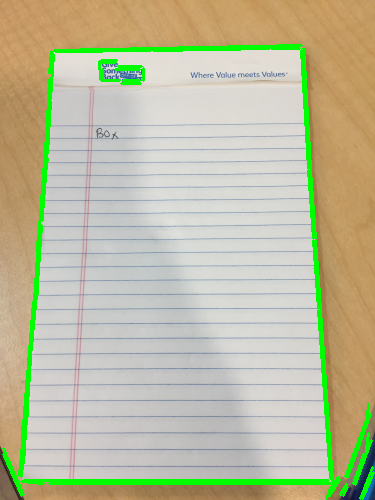
\includegraphics[scale=0.5]{img/perspective/lsd}
    \caption{Найденные на изображении линии с помощью алгоритма $LSD$}
    \label{lsd_img}
\end{figure}

Контур определяется как пересечение горизонтальных и вертикальных линий. На выходе имеем найденные углы контура, показанные на рисунке ~\ref{lsd_corners}
\begin{figure}
    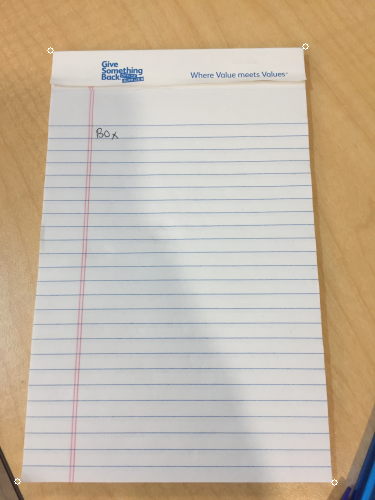
\includegraphics[scale=0.5]{img/perspective/corners}
    \caption{Найденные на изображении контуры на основе линий}
    \label{lsd_corners}
\end{figure}

С помощью библиотеки $openCV$ контуры находятся следующим образом:

\begin{enumerate}
    \item Находятся 5 наибольших по площади контуров
    \item Найденные контуры проверяются на количество углов, минимальную площадь контура
\end{enumerate}

Среди всех подходящих контуров выбирается наибольший по площади, как показано на рисунке ~\ref{contours}
\begin{figure}
    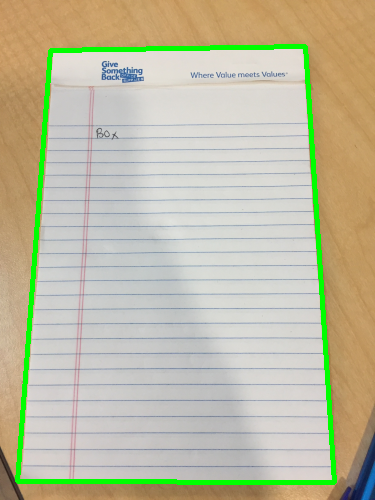
\includegraphics[scale=0.5]{img/perspective/contours}
    \caption{Найденные алгоритмом контуры}
    \label{contours}
\end{figure}


На основе найденного контура, представляющего лист бумаги, осуществляем коррекцию перспективы. Для этого находим матрицу коррекции \cite{opencv_perspective_transform} и примянем ее к изображению \cite{opencv_warp_perspective}.
Получаем результирующее изображение, показанное на рисунке ~\ref{perspective_correction}
\begin{figure}
    \includegraphics[scale=0.1]{img/perspective/perspective}
    \caption{Изображение с коррекцией перспективы}
    \label{perspective_correction}
\end{figure}

Далее необходимо добавить эффект сканирования. Эффект достигается путем применения к композиции небольшого размытия и серого изображения алгоритма сегментации $Adaptive Threshold$ \cite{opencv_threshold}. 
В конечном итоге имеем результирующее изображение показанное на рисунке ~\ref{preprocess_out}

\begin{figure}
    
\includegraphics[scale=0.15]{img/perspective/output}
    \caption{Результирующее изображение}
    \label{preprocess_out}
\end{figure}